\chapter{告発する約束・評判ゲーム}
本章では、\ref{hypothesis}節で定義した補題2を検証する。

\section{補題2}
\secondLemma
% 成員の行動を観察できない外部の強制執行力が存在すると仮定した上で、集団を構成する成員達の性質によっては、
% 成員達に合意された約束を履行させるインセンティブ設計が可能である。

\section{提案手法}
不正行為にあった場合に必ず「失敗」を報告する行動を「告発」と呼び、
「告発」するプレイヤーのみが参加する「約束・評判ゲーム」を「告発する約束・評判ゲーム」とする。
この「告発する約束・評判ゲーム」において、不正が防止される条件を導き出す。
そして、その条件を満たす「評判システム」を通常の「約束・評判ゲーム」に適用し、
様々な戦略をとるエージェントをランダムに用意したマルチエージェントシミュレーションを行ことで、
「告発」するプレイヤーが一定以上存在していれば成員達に合意された約束を履行させることができることを示す。


\section{告発}
\ref{verification1}節の検証では、
「評判システム」は$reporter$が戦略$s_{r1}$と$s_{r4}$をとる確率$p_{r1}$と$p_{r4}$を推定できないため、
不正を防止する「評判スコア」の変化量の組$(r_{ps}, r_{pf}, r_{ps}, r_{pf})$を決定できなかった。
これは$reporter$が報告する約束の結果と真の約束の結果が一致している保証がないためである。
そこで、本論では、$promiser$が約束を反故にした場合に「失敗」を報告する行動を「告発」とする。
この行動をとる成員が多数いれば、先の確率を近似することが可能であると考えられる。
% これまでの研究においても、こうした報復的な行動が道徳的規範の出現に関係することがわかっている。(TODO: 要出典)


\section{告発する約束・評判ゲーム}
「告発」する成員のみで行われる「約束・評判ゲーム」を「告発する約束・評判ゲーム」とする。
このゲームにおいては、step1で$promisor$が約束を履行しなかった場合、$reporter$は必ず「失敗」を報告するため、
図\ref{ethical-gametree}のゲームの木のような展開型ゲームとして表せる。
また、\ref{playersStrategy}節で示した$reporter$の戦略のうち$s_{r2}$と$s_{r4}$がとられないため、
非協力戦略型ゲームとして表したときの利得は表\ref{ethical-gametable}のようになる。
注意すべき点としては、報告された約束の結果が次回以降のゲームで意味のある情報となるため、
「成功」と「失敗」が報告された場合の将来の期待利得$\epsilon$と$\lambda$について考慮する必要がある。

\clearpage
\begin{figure*}
  \centering
  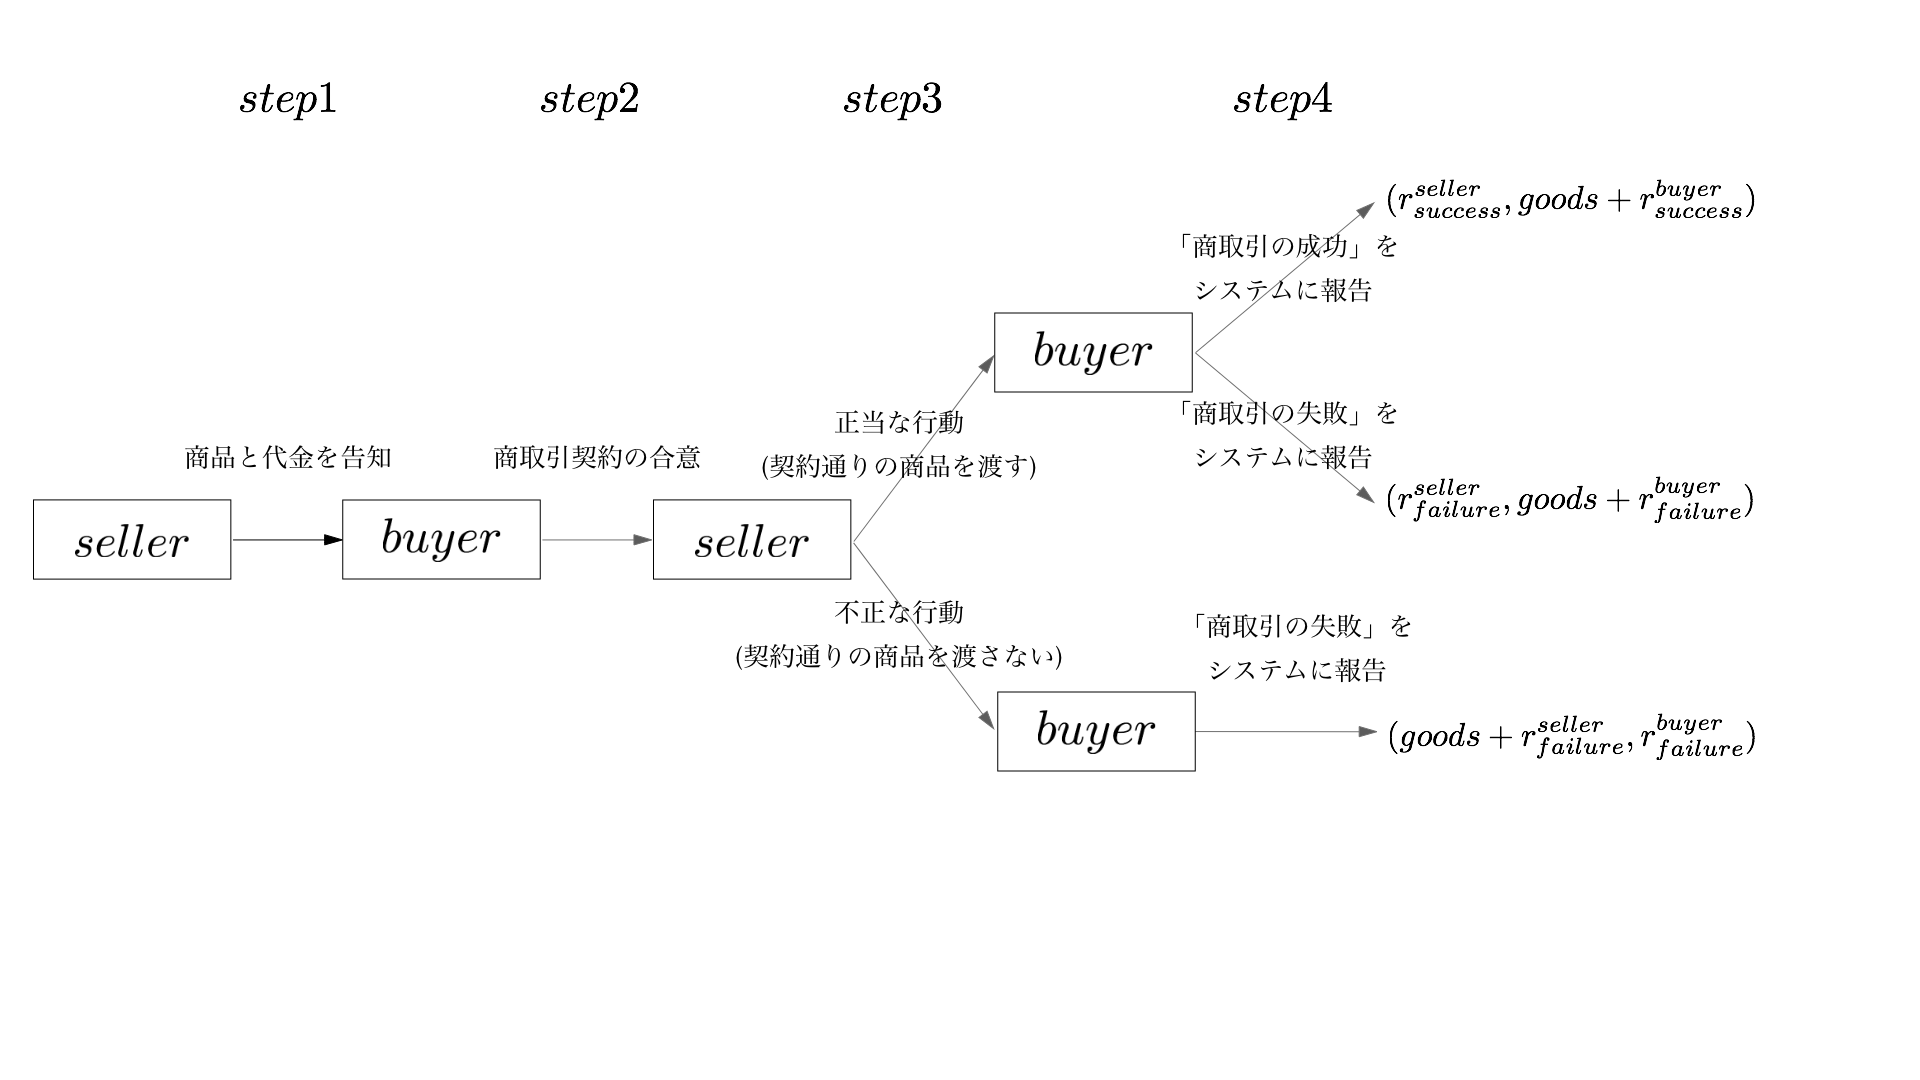
\includegraphics[width=1\linewidth]{./06_ethical-prgame/ethical-gametree.png}
  \caption{「告発する約束・評判ゲーム」のゲーム木}
  \label{ethical-gametree}
\end{figure*}

\subsection{各プレイヤーの戦略}
% \label{playersStrategy}
この展開型ゲームにおける$promisor$と$reporter$の行動は、下記のような戦略として表せる。

\subsubsection{$promisor$の戦略}
\begin{description}
  \item[$s_{p1}$]… 約束を履行する
  \item[$s_{p2}$]… 約束を反故にする
\end{description}

\subsubsection{$reporter$の戦略}
\begin{description}
  \item[$s_{r1}$]… $promisor$が約束を履行した場合は「成功」,反故にした場合は「失敗」を報告する
  \item[$s_{r3}$]… $promisor$が約束を履行した場合は「失敗」,反故にした場合は「失敗」を報告する
\end{description}


% Success Reported on True Success
\newcommand{\SROS}{ $(c_{p1} + r_{ps},$ \\$c_{r1} + r_{rs})$ }
\newcommand{\FROF}{ $(c_{p2} + r_{ps},$ \\$c_{r2} + r_{rs})$ }
\newcommand{\FROS}{ $(c_{p1} + r_{pf},$ \\$c_{r1} + r_{rf})$ }
\newcommand{\SROF}{ $(c_{p2} + r_{pf},$ \\$c_{r2} + r_{rf})$ }
\newcommand{\tabularc}[1]{\begin{tabular}{c} #1 \end{tabular}}

\begin{table*}[h]
  \begin{tabular}{|l|l|l|l|l|l|}
  \hline
  \multicolumn{2}{|l|}{\multirow{2}{*}{}} & \multicolumn{4}{l|}{$Reporter$} \\ \cline{3-6}
  \multicolumn{2}{|l|}{}                  &$s_{r1}$&$s_{r2}$&$s_{r3}$&$s_{r4}$\\ \hline
  \multirow{2}{*}{$Promisor$}
  &$s_{p1}$&\tabularc{\SROS}&\tabularc{\SROS}&\tabularc{\FROS}&\tabularc{\FROS}\\ \cline{2-6}
  &$s_{p2}$&\tabularc{\SROF}&\tabularc{\FROF}&\tabularc{\SROF}&\tabularc{\FROF}\\ \hline
  \end{tabular}
  \caption{「約束・評判ゲーム」の利得票表}
  \label{prgametable}
\end{table*}

\subsection{各変数の定義}
% \label{prgamePayoffVariables}
\begin{description}
  % \centering
  \item[$\epsilon_p$]… 「成功」が報告された場合の$promisor$の将来期待利得
  \item[$\epsilon_r$]… 「成功」が報告された場合の$reporter$の将来期待利得
  \item[$\lambda_p$]… 「失敗」が報告された場合の$promisor$の将来期待利得
  \item[$\lambda_r$]… 「失敗」が報告された場合の$reporter$の将来期待利得
  \item[$c_{p2}$]… 約束が反故にされた場合の$promisor$の「評判スコア」の変化量以外の効用
  \item[$c_{p1}$]… 約束が履行された場合の$promisor$の「評判スコア」の変化量以外の効用
  \item[$c_{p2}$]… 約束が反故にされた場合の$promisor$の「評判スコア」の変化量以外の効用
  \item[$c_{r1}$]… 約束が履行された場合の$reporter$の「評判スコア」の変化量以外の効用
  \item[$c_{r2}$]… 約束が反故にされた場合の$reporter$の「評判スコア」の変化量以外の効用
  \item[$r_{ps}$]… 「成功」が報告された場合の$promisor$の「評判スコア」の変化量
  \item[$r_{pf}$]… 「失敗」が報告された場合の$promisor$の「評判スコア」の変化量
  \item[$r_{rs}$]… 「成功」が報告された場合の$reporter$の「評判スコア」の変化量
  \item[$r_{rf}$]… 「失敗」が報告された場合の$reporter$の「評判スコア」の変化量
\end{description}

\section{不正が防止される条件}
表\ref{prgametable}より,「告発する約束・評判ゲーム」において、約束が履行され「成功」が報告されるためには、
$promisor$と$reporter$のとる戦略組が$ (s_{p1}, s_{r1})$になる必要がある.
各プレイヤーが戦略$s$をとったときの利得を$R$とし、その期待値を$E(R|s)$とする。
全てのプレイヤーが完全に合理的な場合、戦略組$(s_{p1}, s_{r1})$に帰着させるためには,

\begin{description}
  \centering
  \item[条件③] $E(r|s_{p1}) > E(r|s_{p2})$かつ$E(r|s_{r1}) > E(r|s_{r3})$
\end{description}

を満たす「評判スコア」の変化量の組$(r_{ps}, r_{pf}, r_{rs}, r_{rf})$を「評判システム」から決定できる必要がある.

\subsection{各戦略のとられる確率}
各プレイヤーが戦略$s_{k}$をとる確率を$p_{k}$とする.

\begin{gather}
  0 \leq p_{k} \leq 1 \nonumber \\
  p_{p1} + p_{p2} = 1 \label{condition5-1} \\
  p_{r1} + p_{r3} = 1 \label{condition5-2}
\end{gather}

\subsection{各戦略の期待利得}
$promisor$と$reporter$の各戦略の期待利得は次のように表せる.

\begin{eqnarray}
  E(R|s_{p1}) &=& p_{r1} (c_{p1} + r_{ps} + \epsilon_p) + p_{r3} (c_{p1} + r_{pf} + \lambda_p) \nonumber \\
              &=& c_{p1} + p_{r1} (r_{ps} + \epsilon_p) + p_{r3} (r_{pf} + \lambda_p) \because\eqref{condition5-2} \\
  E(R|s_{p2}) &=& p_{r1} (c_{p2} + r_{pf} + \lambda_p) + p_{r3} (c_{p2} + r_{pf} + \lambda_p) \nonumber \\
              &=& c_{p2} + r_{pf} + \lambda_p  \because\eqref{condition5-2} \\
  E(R|s_{r1}) &=& p_{p1} (c_{r1} + r_{rs} + \epsilon_r) + p_{p2} (c_{r2} + r_{rf} + \lambda_r) \\
  E(R|s_{r3}) &=& p_{p1} (c_{r1} + r_{rf} + \lambda_r) + p_{p2} (c_{r2} + r_{rf} + \lambda_r) \nonumber \\
              &=& p_{p1} c_{r1} + p_{p2} c_{r2} + r_{rf} + \lambda_r \because\eqref{condition5-1}
\end{eqnarray}

\subsection{$promiser$が$s_{p1}$をとる条件}

$ E(R|s_{p1}) > E(R|s_{p2}) $を満たすためには、
\begin{eqnarray}
  &&E(R|s_{p1}) > E(R|s_{p2}) \nonumber \\
  &\therefore& c_{p1} + p_{r1} (r_{ps} + \epsilon_p) + p_{r3} (r_{pf} + \lambda_p) > c_{p2} + r_{pf} + \lambda_p \nonumber \\
  &\therefore& p_{r1} (r_{ps} + \epsilon_p) + (p_{r3} - 1) (r_{pf} + \lambda_p) > c_{p2} - c_{p1} \nonumber \\
  &\therefore& p_{r1} (r_{ps} + \epsilon_p) - (1 - p_{r3}) (r_{pf} + \lambda_p) > c_{p2} - c_{p1} \nonumber \\
  &\therefore& p_{r1} (r_{ps} + \epsilon_p) - p_{r1} (r_{pf} + \lambda_p) > c_{p2} - c_{p1} \because\eqref{condition5-2} \nonumber \\
  &\therefore& p_{r1} (r_{ps} - r_{pf} + \epsilon_p - \lambda_p) > c_{p2} - c_{p1}
\end{eqnarray}

を満たせばよい.

\subsection{$reporter$が$s_{r1}$をとる条件}

$ E(R|s_{r1}) > E(R|s_{r3}) $を満たすためには、
\begin{eqnarray}
  &&E(R|s_{r1}) > E(R|s_{r3}) \nonumber \\
  &\therefore& p_{p1} (c_{r1} + r_{rs} + \epsilon_r) + p_{p2} (c_{r2} + r_{rf} + \lambda_r) > p_{p1} c_{r1} + p_{p2} c_{r2} + r_{rf} + \lambda_r \nonumber \\
  &\therefore& p_{p1} (r_{rs} + \epsilon_r) + p_{p2} (r_{rf} + \lambda_r) > r_{rf} + \lambda_r \nonumber\\
  &\therefore& p_{p1} (r_{rs} + \epsilon_r) + (p_{p2} - 1) (r_{rf} + \lambda_r) > 0 \nonumber \\
  &\therefore& p_{p1} (r_{rs} + \epsilon_r) - (1 - p_{p2}) (r_{rf} + \lambda_r) > 0 \nonumber \\
  &\therefore& p_{p1} (r_{rs} + \epsilon_r) - p_{p1} (r_{rf} + \lambda_r) > 0 \because\eqref{condition5-1} \nonumber \\
  &\therefore& p_{p1}(r_{rs} - r_{rf} + \epsilon_r - \lambda_r) > 0
\end{eqnarray}

を満たせばよい。


\subsection{戦略組($s_{p1}$, $s_{r1}$)に帰結する条件}

$p_{r1} > 0$かつ $p_{p1} > 0$かつ$ \epsilon_p > \lambda_p $かつ$ \epsilon_r > \lambda_r $を仮定すると\\

\begin{equation}
  r_{ps} - r_{pf} \geq \frac{c_{p2} - c_{p1}}{p_{r1} } \label{conditionByPr1}
\end{equation}

かつ

\begin{equation}
  r_{rs} - r_{rf} \geq 0
\end{equation}

を満たせば,「告発する約束約束・評判ゲーム」で不正を防止することができる.

\subsection{戦略$s_{p1}$をとった割合と成功が報告される割合の関係}
% メモ:要修正
全ての成員は「告発」するため、
任意の成員$i$と$j$のこれまでの「約束・評判ゲーム」で$s_{p1}$をとってきた割合$FulfillStrategyRate(i, j)$と、
「評判システム」に報告された約束の記録のうち
$promisor$が成員$i$で$reporter$が成員$j$である記録の「成功」の割合$ReportedSuccessRate(i, j)$について、次の関係がいえる。

\begin{equation}
  FulfillStrategyRate(i, j) \geq ReportedSuccessRate(i, j) \label{inequalityFR}
\end{equation}


\subsection{信頼度 $ P_i $}

ここで、成員$i$が$promisor$のときに$s_{p1}$をとる確率$ p_{p1} $を成員$i$の信頼度$P_i$と定義し,
$ P_i $を$FulfillStrategyRate(i, j)$と$\sum^{\{1, 2, ..., n\}}_{k}w_k = 1$を満たす
任意の重み$ w_k $ ($k \in \{1, 2, ..., n\}$)を用いた荷重総和として次のように表す. \\

\begin{eqnarray}
  P_i &\equiv& p_{p1} \\
      &\equiv& \sum^{\{1,2,..., n\}}_{j} w_{j} \cdot FulfillStrategyRate(i, j)
\end{eqnarray}


\subsection{最低信頼度 $ T_i $}
また、$ ReportedSuccessRate(i, j)$に、同じ重み$ w_k $を用いた荷重総和を最低信頼度$ T_i $と定義する. \\

\begin{equation}
  T_i \equiv \sum^{\{1,2,..., n\}}_{j} w_j \cdot ReportedSuccessRate(i, j) \label{conditionT_i}
\end{equation}

\subsection{最低信頼度$T_i$を用いた条件}

\eqref{inequalityFR}より、$ P_i \geq T_i $がいえるため、\eqref{conditionByPr1}について

\begin{eqnarray}
  r_{ps} - r_{pf} &\geq& \frac{c_{p2} - c_{p1}}{T_i} \\
                  &\geq& \frac{c_{p2} - c_{p1}}{P_i} = \frac{c_{p2} - c_{p1}}{p_{r1}} \nonumber
\end{eqnarray}

がいえる.\\

「評判システム」から最低信頼度$T_i$は既知のため、
$p_{r1} > 0$かつ $p_{p1} > 0$かつ$ \epsilon_p > \lambda_p $かつ$ \epsilon_r > \lambda_r $を仮定した上で,
「告発する信用・評判ゲーム」において、不正を防止する$ (r_{ps}, r_{pf}, r_{rs}, r_{rf}) $の組を「評判システム」から決定できる。

\section{評判システムの詳細}
本節ではシミュレーションに用いる「評判システム」の仕様の詳細を紹介する。
完全な実装については、GitHubのソースコードを参照。

\subsection{約束の価値$C$}
\begin{eqnarray}
  C &\equiv& 1 \\
    &=& c_{p2} - c_{p1} \\
    &=& c_{r1} - c_{r2}
\end{eqnarray}

\subsection{ReputationWeight}
最低信頼度$ T_i $を求めるため、$ReportedSuccessRate(i, j)$の荷重総和に用いる重み$ w_k $を定義する.
この重み$w_k$は、任意の成員$i$が戦略$s_{p1}$をとる確率$p_{p1}$を推定する際に、
成員$i$と他の成員$j$における$ReportedSuccessRate(i, j)$をどの程度信頼するかを表している。
本実験では、成員$j$の「評判スコア」が全体に占める割合をReputationWeight$w_j$と定義する。
任意の成員$k$の「評判スコア」を$b_k$としたとき、$w_k$は次のように表せる。($n$は成員の人数)

\begin{equation*}
  w_k \equiv \frac{b_k}{\sum^{\{1,2,...,n\}}_{k}b_k}
\end{equation*}

\subsection{「成功」が報告された場合の「評判スコア」の変化}
$ reporter $が「成功」を報告した場合、
$ reporter $は約束の価値$C$だけ減り、$ promisor $は$C$だけ増加するものとする。

\begin{gather}
  r_{ps} = C \\
  r_{rs} = -C \\
  r_{ps} + r_{rs} = 0
\end{gather}


\subsection{EscrowCost}
「失敗」が報告されたとき、$promisor$と$reporter$が失う「評判スコア」の合計を$EscrowCost$とする。
約束の価値$C$にエスクロー係数$E$を掛けたものとする.

\begin{eqnarray}
  EscrowCost  &\equiv& (r_{rs} - r_{rf}) + (r_{ps} - r_{pf}) \\
              &=& E \cdot C \label{escrowCost}
\end{eqnarray}

\subsection{EscrowCostの負担比率}
成員$i$を$promiser$、$j$を$reporter$とする。
「約束・評判ゲーム」を行うとき、$EscrowCost$の負担比率を両者の最低信頼度$T_i$を用いる.\\

\begin{equation}
  (r_{ps} - r_{pf}):(r_{rs} - r_{rf}) = T_j:T_i
\end{equation}

\subsection{EscrowCostの分配}
「失敗」が報告されたときに$EscrowCost$が消失すると、
「評判スコア」の総量が下がり、約束の価値$C$

総量を一定に保つために、$promisor$と$reporter$以外の全てのプレイヤーに、
$ReputationWeight$に応じて$EscrowCost$を分配する。
$promisor$と$reporter$を含まないのは、分配によるインセンティブ設計への影響をなくすためである。

\subsection{不正が防止される条件を満たす定義}
成員$j$を$promiser$、$k$を$reporter$とする。
このとき、\eqref{condition6-1}と\eqref{condition6-2}を満たす$r_{ps} - r_{pf}$と$r_{rs} - r_{rf}$を下記のように定義する。

\begin{eqnarray}
  r_{ps} - r_{pf} &\equiv& \frac{C}{T_i} \label{condition6-3} \\
                  &\geq& \frac{c_{p2} - c_{p1}}{T_i} \nonumber \\
  r_{rs} - r_{rf} &\equiv& \frac{C}{T_j} \label{condition6-4} \\
                  &\geq& 0 \nonumber
\end{eqnarray}

\subsection{残高の変化量の組$ (r_{ps}, r_{pf}, r_{rs}, r_{rf}) $}
上記の定義からエスクロー係数$E$と残高の変化量の組$ (r_{ps}, r_{pf}, r_{rs}, r_{rf}) $は次のように求まる. \\
成員$i$を$promisor$、$j$を$reporter$とする。

\begin{eqnarray}
  E &=& - \frac{T_i + T_j}{T_i T_j} \\
  r_{ps} &=& 1 \\
  r_{pf} &=& 1 - \frac{1}{T_j} \\
  r_{rs} &=& -1 \\
  r_{rf} &=& -1 - \frac{1}{T_i}
\end{eqnarray}


\section{実験方法}
先の不正が防止される条件を満たすインセンティブ設計を行う「評判システム」と
次の8タイプのエージェントから重複問わずランダムに選んだ8体のエージェントを用意し試行を実施する。
これをタイプAのエージェントが0〜7体を占める場合について、それぞれ8000回づつ繰り返し、
エージェントの構成とstep13で求まる「報告された成功率」と「真の成功率」を記録する。

\subsection{エージェントの種類}
下記のA~Hの8タイプのエージェントを用意する。
\begin{description}
  \item [A] 約束を履行し、$promisor$が約束を履行したとき「成功」、反故にしたとき「失敗」を報告する。
  \item [B] 約束を履行し、$promisor$が約束を履行したとき「成功」、反故にしたとき「成功」を報告する。
  \item [C] 約束を履行し、$promisor$が約束を履行したとき「失敗」、反故にしたとき「成功」を報告する。
  \item [D] 約束を履行し、$promisor$が約束を履行したとき「失敗」、反故にしたとき「失敗」を報告する。
  \item [E] 約束を反故にし、$promisor$が約束を履行したとき「成功」、反故にしたとき「失敗」を報告する。
  \item [F] 約束を反故にし、$promisor$が約束を履行したとき「成功」、反故にしたとき「成功」を報告する。
  \item [G] 約束を反故にし、$promisor$が約束を履行したとき「失敗」、反故にしたとき「成功」を報告する。
  \item [H] 約束を反故にし、$promisor$が約束を履行したとき「失敗」、反故にしたとき「失敗」を報告する。
\end{description}

\subsection{試行}
\begin{description}
  \item[step 1] 時刻tを0とする。
  \item[step 2] 「評判システム」の各エージェントの初期の「評判スコア」を8とする。
  \item[step 3] 全てのエージェントが$promisor$と$reporter$として1度ずつ総当りする順序を決定する。(順序の長さは56となる)
  \item[step 4] 時刻tを1進める。
  \item[step 5] step 3で決定した順序を周期として、$promisor$と$reporter$を決定する。
  \item[step 6] 「評判システム」は「成功」と「失敗」が報告された場合の$promisor$と$reporter$の「評判スコア」を計算する。
  \item[step 7] $promisor$は自身の戦略に基づいて約束を履行するか反故にする。
  \item[step 8] $reporter$は自身の戦略とstep 6の$promisor$の行動に基づいて結果を決定する。
  \item[step 9] $reporter$は決定した結果を「評判システム」に報告する。 
  \item[step 10] 「評判システム」はstep6で計算した「評判スコア」がいずれの場合にも0未満にならない場合、 reporterから報告された結果を記録する。
  \item[step 11] step6で計算した「評判スコア」がいずれの場合にも0未満にならない場合、真の結果を記録する。
  \item[step 12] 時刻tが1120未満なら、step4に戻る。
  \item[step 13] 過去56回の約束・評判ゲームにおいて、step10と11で記録された結果を集計し、それぞれ「報告された成功率」と「真の成功率」を記録する。
\end{description}

\section{評価}
先の実験の結果、「報告された成功率」と「真の成功率」の両方が100\%になった場合を「不正防止の成功」とし、
誠実なエージェント(タイプA)の数と「不正防止の成功」に至った割合をプロットしたものが、図\ref{ethical-game-001}である。
(エージェント数8の場合は、エージェントの組み合わせが1通りしか存在しないため、個別に試行を行い結果を集計している。)
誠実なエージェントの数が0体の場合であっても不正が防止される構成が存在し、
6体以上の場合はサンプリングした全ての構成で不正の防止が成功していた。

\begin{figure}[h]
  \begin{tabular}{cc}
    \begin{minipage}[t]{1\hsize}
      \centering
      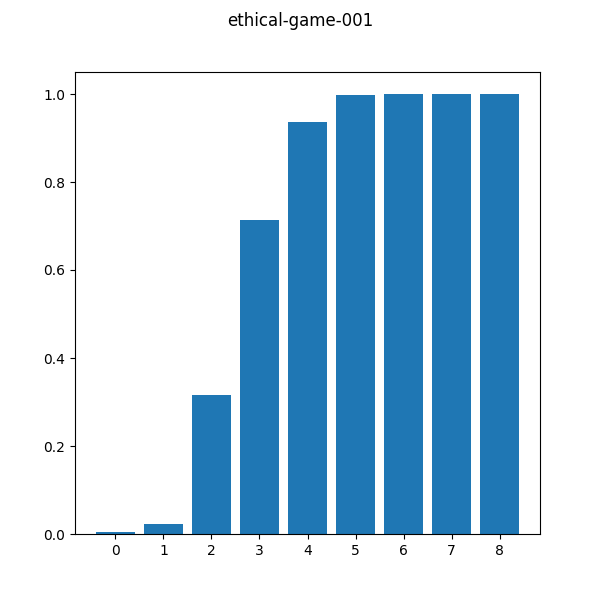
\includegraphics[keepaspectratio, width=1\linewidth]{./06_ethical-prgame/ethical-game-001.png}
      \caption{誠実なエージェントの数と「不正防止の成功」に至った割合}
      \label{ethical-game-001}
    \end{minipage}
  \end{tabular}
\end{figure}

\section{結論}
実験とその評価から、「告発」という限定合理性を仮定した上で「評判スコア」の変化量を決定することで、
成員の構成によっては「約束・評判ゲーム」において不正を防止することができるとわかった。
これによって補題2は示される。
また、成員の構成と不正防止の成功成功の関係性については、先の実験の図\ref{ethical-game-001}のとおりである。
